% Author: Ozgur Taylan TURAN
% Delft University of Technology
\documentclass{article}

\usepackage{/home/taylanot/texmf/tex/arxivtemplate}

\usepackage[utf8]{inputenc} % allow utf-8 input
\usepackage[T1]{fontenc}    % use 8-bit T1 fonts
\usepackage{hyperref}       % hyperlinks
\usepackage{url}            % simple URL typesetting
\usepackage{booktabs}       % professional-quality tables
\usepackage{amsfonts}       % blackboard math symbols
\usepackage{nicefrac}       % compact symbols for 1/2, etc.
\usepackage{microtype}      % microtypography
\usepackage{lipsum}
\usepackage{graphicx}
\usepackage{tikz}
\usepackage{caption}
\usepackage{float}
\usepackage{subcaption}
\usepackage{algorithm2e}
\usepackage{algpseudocode}
\usepackage{wrapfig}
\usetikzlibrary{external}
\tikzexternalize[prefix=Figures/tikz]
\newcommand{\includetikz}[2]{ \resizebox{#1}{!}{\input{#2}}}
\usepackage{amssymb}
\usepackage{mathrsfs}
\usepackage{pgfplots}
%\usepackage{float}
%\usepackage[cochineal,bigdelims,cmintegrals,vvarbb]{newtxmath}
\usepackage{amsmath}       % blackboard math symbols
\usepackage{bm}       % blackboard math symbols
\usepackage[cal=cm]{mathalfa}

% problem
\newcommand{\ispace}{\mathbb{X}}
\newcommand{\ospace}{\mathbb{Y}}
\newcommand{\hypspace}{\mathbb{H}}
\newcommand{\hyp}{h}
\newcommand{\inp}{x}
\newcommand{\out}{y}
\newcommand{\algo}{\mathcal{A}}
\newcommand{\nsamp}{N}
\newcommand{\nsampi}{N_i}
\newcommand{\samp}{\mathcal{D}_\nsamp}
\newcommand{\sampi}{\mathcal{D}_{\nsamp_{i}}}
\newcommand{\prob}{\mathcal{P}}
\newcommand{\probspace}{\mathbb{P}}
\newcommand{\pred}{\hat{y}}
\newcommand{\loss}{\mathcal{L}}
\newcommand{\risk}{\mathcal{R}}
\newcommand{\avgrisk}{\bar{\risk}}
\newcommand{\expect}{\mathbb{E}}
\newcommand{\Zpos}{\mathbb{Z^+}}
\newcommand{\R}{\mathbb{R}}
\newcommand{\task}{\mathcal{T}}

\newcommand{\algolr}{\mathbb{M}}
\newcommand{\lc}{\mathcal{C}}
\newcommand{\nlim}{k}
\newcommand{\nsamplr}{Q}
\newcommand{\numlc}{M}
\newcommand{\samplr}{\mathcal{Z}}
\newcommand{\model}{\mathcal{M}}
\newcommand{\hilbert}{\mathbb{H}}
\newcommand{\data}{\boldsymbol{\alpha}}
\newcommand{\func}{\boldsymbol{\beta}}

%\newcommand{\slope}{\mathbf{w}}
%\newcommand{\bias}{b}
%\newcommand{\task}{\mathcal{T}}
%\newcommand{\dataset}{\mathcal{Z}}
%\newcommand{\scaletask}{\mathbf{a}}
%\newcommand{\inpbias}{\bar{\mathbf{x}}}
%\newcommand{\phasetask}{\boldsymbol{\phi}}
%\newcommand{\lab}{y}
%\newcommand{\labs}{\mathbf{y}}
%\newcommand{\EE}{\mathcal{E}}
%\newcommand{\trainset}{Z}
%\newcommand{\model}{\mathcal{M}}
%\newcommand{\estim}{\mathcal{\hat{M}}}
%\newcommand{\noise}{\varepsilon}
%\newcommand{\var}{\sigma^2}
%\newcommand{\mean}{\mu}
%\newcommand{\ridge}{\lambda}
%\newcommand{\kernel}{\kappa}
%\newcommand{\weight}{\boldsymbol{\alpha}}
%\newcommand{\genridge}{\mathbf{h}}
%\newcommand{\normal}[2]{\mathcal{N}(#1, #2)}
%\newcommand{\param}{\bar{\mathbf{w}}}
%\newcommand{\opt}{\mathbf{\hat{\bar{w}}}}
% GD
\newcommand{\iter}{n_{{iter}}}
\newcommand{\lr}{\eta}
\newcommand{\grad}[1]{\nabla_{#1}}
%\newcommand{\loss}{\mathcal{L}}
% math
\newcommand{\trans}[1]{#1^\text{T}}
\newcommand{\inv}[1]{#1^{-1}}
\newcommand{\sine}{\text{sin}}
\newcommand{\norm}[2]{||#1||_#2}

% matrix
\newcommand{\design}{{\mathbf{X}}}
\newcommand{\gram}{{\mathbf{K}}}
\newcommand{\ones}{\mathbf{1}}
\newcommand{\zeros}{\mathbf{0}}
\newcommand{\I}{\mathbf{I}}

% Text Related Commands
\newcommand{\eg}{\textit{e.g.}}

%% Title
%\title{Expected Loss of MAML:A Comperative Study}
\title{Learning "Learning Curves"}
%%%% Cite as
%%%% Update your official citation here when published 
%\thanks{\textit{\underline{Citation}}: 
%\textbf{Authors. Title. Pages.... DOI:000000/11111.}} 


\author{
  Author1, Author2 \\
  Affiliation \\
  Univ \\
  City\\
  \texttt{\{Author1, Author2\}email@email} \\
  %% examples of more authors
   \And
  Author3 \\
  Affiliation \\
  Univ \\
  City\\
  \texttt{email@email} \\
  %% \AND
  %% Coauthor \\
  %% Affiliation \\
  %% Address \\
  %% \texttt{email} \\
  %% \And
  %% Coauthor \\
  %% Affiliation \\
  %% Address \\
  %% \texttt{email} \\
  %% \And
  %% Coauthor \\
  %% Affiliation \\
  %% Address \\
  %% \texttt{email} \\
}
% For version 1 
%\newcommand{\version}{v1/}
% For version 2 
\newcommand{\version}{v1/}
\graphicspath{{Figures_\version/}}     % organize your images and other figures under media/ folder
\begin{document}
\maketitle


\begin{abstract}
  Model-Agnostic Meta-Learning is a meta-learning method that achieved state-of-the-art performance few-shot image classification benchmarks at the time of its introdction. MAML's primary novelties lies with it being applicable to any gradient based model and allowing quick adaptation to a new task in time-critical settings. Although, there is no need for a quick adaptation in most of the few-shot learning benchmarks, MAML is still being utilized as a benchmark for derivative/follow-up work. This raises the question what does MAML add in those settings where the quick adaptation is not bestowed by the problem. In this intial study we aim to investigate the expected performance of the MAML compared to some conventional base learners for synthetic linear and nonlinear regression problems. 



\end{abstract}


% keywords can be removed
\keywords{meta-learning \and expected performance \and learning-curves \and functional analysis}

\section{Introduction}\label{sec:intro}
  
% Meta Learning Definitions
Learning to learn, also referred to as meta-learning, treats the training of a machine learning model as a learning problem in itself. In the context of this work if a machine learning model's performance on a task is improving with training experiences it is said to be learning. In the light of this definition a machine learning model is said to be learning to learn if the performance on each task improves with training experience obtained from each task and with the number of tasks \cite{thrun1998}. Meta-learning recently is being used to tackle few-shot learning problems, where there is little data available from the learning task that is of prime interest, whereas there is an abundance of data from other similar tasks. 

% What Makes MAML Different
Early works of the learning-to-learn paradigm relied upon the one supervisory and one sub-ordinate model that interacts with each other for meta-learning. On one hand, sub-ordinate models try to improve the performance with training examples and on the other hand, the supervisory model tries to increase the performance over the family of tasks. MAML (Model-Agnostic Meta-Learning) \cite{finn2017} is a model that circumvents the need for supervisory and subordinate models. This method tries to tackle meta-learning by training any (As the name suggests MAML applies to all learners that improve performance by SGD (Stochastic Gradient Descent).) machine learning models parameters in a way to maximize the performance on a new learning task with few experiences through one or more gradient steps. 

% Where to use MAML?
MAML is used in few-shot learning problems in the supervised and reinforcement learning problems, where the losses differ from each other. Due to being model and problem independent MAML finds a wide application area in the context of few-shot meta-learning. Moreover, MAML also aims to improve a specific task performance quickly (with a few gradient steps). This is an additional aspect to our definition of meta-learning. 

% What is the problem?
As mentioned above, MAML aims to improve the generalization of a model for a certain learning task from a given family of tasks, with little data and minimal training. Minimal training indicates quick adaptation capabilities. This feature can prove useful in certain settings, for instance, in robotics research, where the reaction/adaptation time of the agents to dynamic environments bestow an inherent time limitation. However, this limitation is not present for the supervised learning problems, where MAML or its variants are utilized as a baseline. (\eg \cite{flennerhag2019, nichol2018, rajasegaran2020, collins2020, guiroy2019} etc.) Most of the unsupervised problem benchmark is image detection problem, where $N$-way $K$-shot classification problem ($N$ different classes with $K$ labeled training data) is tried to be tackled. Given the nature of the problem, most of the time memory or time limitation does not constitute a major issue in the given problem setting.

% What is our paper about?
The main aim of this paper is to investigate the MAML under the settings where quick adaptation is not needed, and where most of the applications and variants of this method are benchmarked. This will be achieved by looking at the expected performance of the MAML under 2 regression scenarios, and comparing its performance to conventional base learners (\eg Linear Regression, Ridge Regression, Kernel Ridge Regression, etc.). By doing this we aim to investigate the effect of the limited adaptation step.% In the meantime, the effect of task variance, and noisy observations (unlike the setting presented in \cite{finn2017}) will also be investigated.



\section{Related Work}\label{sec:rw}
  \begin{itemize}
  \item Database creation.
  \item Non-monotonicity of learning curves
  \item Learning curve approximation methods.
  \item Surveys.
  \item Meta-learning learning curves. (Leiden People)
  \item Have not seen anyone doing something like this yet. But talk about the semi-parametric kernel ridge and its applications.
  \item Maybe ties to structured learning and meta-learning if it does not hinder the flow of the paper.
\end{itemize}

\section{Problem Setting}\label{sec:prob}
  \section{Aim}

\begin{frame}{Aim-\only<1>{A}\only<2>{B}}
\only<1>{
  \begin{minipage}{0.5\textwidth} 
    \includegraphics[width=\textwidth]{Figures/literature/FE2-ML.pdf}
  \end{minipage}%
  \begin{minipage}{0.5\textwidth} 
    \includegraphics[width=\textwidth]{Figures/problem/models.pdf}
  \end{minipage}
}
\only<2>
{
  \begin{minipage}{0.3\textwidth} 
    \centering
    \includegraphics[width=\textwidth]{Figures/problem/collective.pdf}
  \end{minipage}%
  \begin{minipage}{0.7\textwidth} 
    \centering
    \includegraphics[width=\textwidth]{Figures/problem/material.pdf}
  \end{minipage}
}
\end{frame}

\begin{frame}{Overall Learning Problem-\only<1>{A}\only<2>{B}}
  \only<1>
{
  \color{Pink} Consider an arbitrary space that represents overall material behaviour, and the subsets of this space representing specific material types.
  \centering
  \includegraphics[width=0.6\textwidth]{Figures/problem/tasks}
}
  \only<2>
{
  \centering
  \includegraphics[width=0.5\textwidth]{Figures/problem/tasks_example}

  \begin{itemize}
  \item \color{Pink} Every label in this space becomes a full mapping! ( $T_{D_1}:=\{T_{{D_1}_i}:\mathbf{F}\to\mathbf{P}_i\}_{i=1}^M$)
  \end{itemize}
}
\end{frame}



\section{Methods}\label{sec:meth}
  Throughout this work uppercase bold letters (\eg $\mathbf{X}$), lowercase bold letters (\eg $\mathbf{x}$), and lowercase letters (\eg ${x}$) are used for matrices, vectors, and scalars respectively. Moreover, the vectors are assumed to be stored in columns. Finally, the $\I_{D}$ represents a $D\times D$ identity matrix, the $\ones_{D}$ and $\zeros_{D}$ represents $D\times 1$ vector of ones and zeros respectively.

\subsection{Learning Problems}

In this work, two families of regression tasks are considered; a linear and a nonlinear regression task family.

% Maybe we can explain why we choose these...

Consider the conventional linear regression problem

\begin{equation}\label{eq:linearreg}
  \lab = \trans{\inp}\scaletask+\noise, 
\end{equation}
where $\lab\in\R$, $\inp\in\R^D$, $\scaletask\in\R^D$ and $\noise\sim\normal{0}{\var}$. Each realization of the slope $\scaletask$ corresponds to a task $\task$ and the collection of $N$ observations is represented by $\dataset:=\{\inp_i, \lab_i\}_{i=1}^{N}$. 

For the nonlinear problem family, the regression function is defined as a weighted combination of sinusoidal functions:

\begin{equation}\label{eq:nonlinearreg}
  \lab = \trans{\sine(\inp+\phasetask)}\scaletask+\noise, 
\end{equation}
where $\lab\in\R$, $\inp\in\R^D$, $\scaletask\in\R^D$ and $\noise\sim\normal{0}{\var}$. Assuming that the each realization of scale term $\scaletask$ and $\phasetask$ corresponds to a task observed in the environment $\task$ and each set of observed $N$ input ($\inp$) and its corresponding label ($\lab$) is represented by a dataset $\dataset:=\{\inp_i, \lab_i\}_{i=1}^{N}$.

%For both linear and nonlinear problems presented sample distribution is given by $\prob_\dataset$ for a given $\task$ and the task, distribution is represented by $\prob_\task$. 
A model parameterized by $\param$ is represented by $\model(\inp, \param):\inp\to\lab$. A model $\model(\inp, \param)$ that is trained with $\dataset$ obtained from  task $\task$ is represented by $\estim(\inp)$. Noting that $\estim(\inp)$ for a base learner is only exposed to a single task $\task$ and a single dataset $\dataset$, whereas a meta learner, in this case, MAML, are exposed to multiple tasks from $\prob_\task$ and multiple datasets $\dataset$ in the meta-learning stage and then the adaptation is done as in the case of a base learner with just a single task $\task$ and a single dataset $\dataset$.  The discrepancy between the prediction of the estimator $\estim$ and $\lab$ is measured in terms of squared loss $\loss:=(\estim(\inp)-\lab)^2$. The main loss that this paper tries to investigate is the \textit{Expected Squared Loss} of an estimator $\estim$ over the $\prob_{\task}$. Then the expected squared loss can be represented as

\begin{equation}\label{eq:ee}
  \EE:= \iiint(\estim(\inp) - y)^2\prob(\inp, y)\prob_{\dataset}\prob_{\task} d\inp d\lab d\dataset d\task.
\end{equation}

% Maybe this can be elaborated!

This performance measure gives rise to the \textit{Bayes Error} to be given by $\sigma^2$ that is coming from the noise term, which represents a model that is the perfect estimator, referred to as oracle in some of the meta-learning literature.

For all the problems the input distribution is given by $\prob_\inp\sim\normal{0}{k\I}$ where $k$ is a parameter for the variance of the inputs. For the linear problem the $\prob_\task:=\prob(\scaletask)\sim\normal{{m\ones_{D}}}{{c\I_{D}}}$ and for nonlinear problem the task distribution takes the form of a joint distribution $\prob_\task:=\prob(\scaletask, \phasetask)$ where $\prob_{\scaletask}\sim\normal{\ones_{D}}{c_1\I_{D}}$ and $\prob_{\phasetask}\sim\normal{\zeros_{D}}{c_2\I_{D}}$

\begin{figure}[ht!]
  \centering
  \begin{subfigure}[b]{0.49\textwidth}
    \centering
    \includetikz{\textwidth}{Figures_v1/methods/lin_maml.tikz}
    \caption{$\lab = \trans{\inp}\scaletask$}
    \label{fig:lintasks}
  \end{subfigure}
  \begin{subfigure}[b]{0.49\textwidth}
    \centering
    \includetikz{\textwidth}{Figures_v1/methods/nonlin_maml.tikz}
    \caption{$\lab = \trans{\sine(\inp+\phasetask)}\scaletask$}
    \label{fig:nonlintasks}
  \end{subfigure}
  \caption{100 sample tasks drawn from $\prob_\task$ for both linear ($m=0$ and $c=1$) and nonlinear ($c_1=1$ and $c_2=1$) problems with low opacity and the intermediate models for MAML trained with respective $\prob_\task$.}
\end{figure}

\subsection{Models} 

For the linear problems $\model(\inp, \param):=\inpbias\param$ with $\inpbias\in\R^{1\times D+1}$ and $\param\in\R^{D+1\times 1}$ where $\param:=\trans{[\slope, \bias]}$ and $\inpbias:=[\inp, 1]$ is utilized. The optimum parameters ($\opt$) for different linear models are obtained as follows:

\paragraph{Linear Estimator} is given by the least-squares solution, $\opt:=(\inv{\trans{\design}\design)}\trans{\design}\labs$, where $\design\in\R^{N\times D}$ is the design matrix where the observed input data is stored in rows.

\paragraph{Ridge Estimator} is given by $\opt:=(\inv{\trans{\design}\design+\ridge \I_{D})}\trans{\design}\labs$ which is obtained by minimizing the squared loss with the additional term of $\ridge\norm{\param}{2}^2$. %Thus, overall loss takes the form $\loss+\ridge\norm{\param}{2}^2$.

\paragraph{Kernel Ridge Estimator} is given by $\opt= \trans{\design}\weight$ where $\weight:=\inv{(\gram+\ridge\I_{N})}\lab$ where $\gram\in\R^{N\times N}$ is the  \textit{Gram Matrix} obtained by replacing $\trans{\design}\design$ inner product by a kernel $\kernel(\design, \design)$. Then, the prediction of the estimator takes the form $\estim(\pred,\param)=\trans{\weight}\kernel(\pred,\design)$ where $\pred\in\R^{D\times 1}$.

For both linear and nonlinear models, gradient descent can be utilized to update the parameters of a model $\model$. Then,

\paragraph{Gradient Descent} for any given model $\model(\inp, \param)$ and a given number of iterations $\iter$ the gradient descent estimator is given by $\{\param_{j+1}=\param_{j} - \lr\sum_i^{N}\inp_i(\model(\inp,\param_j)-\lab_i)\}_{j=0}^{\iter}$. In other words for any given value of $\param$ one gradient update is given by the gradient with respect to $\param$ with a scaling parameter $\lr$. 

All the models investigated can be divided into two sub-categories the models that have information regarding the task space and the ones that have not. The labels  used in Section \ref{sec:resdis} of the models that have information regarding the task space are as follows:
\begin{itemize}
  \item \textbf{MAML} (for linear problem): corresponds to gradient descent with $\iter$ with the adjustable parameters obtained from the mean of the tasks $\mathbb{E}[\prob_{\task}]$ with small perturbation $\delta\sim\normal{\zeros}{0.1\I}$ since the MAML procedure for a linear model goes to the mean of the task distribution. 
  \item \textbf{MAML} (for nonlinear problem): an intermediate model trained with the network and meta-learning procedure  given in \cite{finn2017} for the sinusoidal regression problem. After which gradient descent with $\iter$ is used for adaptation to a certain task.
\end{itemize} 

Finally, the following model labels have information from a single task:
\begin{itemize}
  \item \textbf{Linear}: standard least squares solution.
  \item \textbf{Ridge}: standard least squares solution with $L_2-regularization$.
  \item \textbf{random GD}: gradient descent with $\iter$ with the adjustable parameters starting from random initialization.
  \item \textbf{Kernel Ridge}: kernelized (with Radial Basis Function Kernel) 
\end{itemize}

For the linear problem setting, it should be noted that the optimum can always be reached when the gradient descent is utilized with an infinitely small learning rate and an infinite number of gradient steps. Thus, allowing us to investigate the difference between taking limited steps or allowing the model to go towards the optimum directly.

It should be noted that the hyper-parameters of the utilized models, if there are any, are selected with a simple grid search with 20 different values and only the one with the lowest mean expected performance over the parameter under investigation is presented in the results. 

\section{Results and Discussion}\label{sec:resdis}
  \subsection{Learning Monotone Learning Curves}

\subsubsection{Learning curve prediction for changing hyper-parameters of the same model and same dataset}\label{sec:same}
\begin{itemize}
  \item The results of this experiment I have already shown. 
  \item It is possible to extrapolate with little error
  \item Needs to write the experimentation one last time in a reproducible way.
\end{itemize}
\subsubsection{Learning curve prediction for tuned hyper-parameter of the same model and different datasets}\label{sec:diff-dataset}
\begin{itemize}
  \item We do not have it yet but after the Section \ref{sec:same} experiments are written again it will be easy to obtain.
  \item I suspect this will be a bit more problematic as the tuned curves have a bit different variations.
\end{itemize}

\subsection{Learning Non-monotone Learning Curves}
\begin{itemize}
  \item We have linear ridge regression for varying lambdas which is non-monotonic.
  \item This method was able to fairly accurately predict even bimodal curves. (Bimodality comes from the different dimensional datasets.
  \item I will take these from Tom. After he comes back he will prepare the already existing non-monotonic examples.
\end{itemize}

\subsection{Performance against baselines}
\begin{itemize}
  \item Here the prediction performance for power-law etc. will be provided.
  \item The difference between the non-monotonic and monotonic predictions will be highlighted.
\end{itemize}


\section{Conclusion}\label{sec:conc}
  Upon our investigation, it is found empirically that meta-information about the task-space can help the generalization performance in linear and nonlinear problem settings. It is found out that the MAML variant methods are superior under certain conditions. It is observed that the gradient-based meta-learning method MAML is only capable performing better only when the task distribution variance is small, compared to regularization-based meta-learning models. Moreover, it is shown that limiting gradient descent steps taken can be beneficial due to the regularizing effect in both linear and nonlinear problem setting. 

Comparing the meta-regularization information utilization via biased regularization provided in \cite{Denevi2018a} has clear advantages in linear problem setting, when compared to meta-information inclusion via training an intermediate model presented in \cite{Finn2017}. Looking at the performance of the biased regularization (\eg General Ridge model) observation including the single task learning performance of the Kernel Ridge regression for the selected investigations, begs the question; "If we can, somehow, incorporate information regarding the task distribution, can we come up with a simpler kernelized and convex model to achieve a more competing method?". Investigation of this type of method is especially interesting for the reasons of explainability and the ease of theoretical understanding compared to models which have non-convex loss spaces.


\section*{Acknowledgments}
%Bibliography
\bibliographystyle{unsrt}  
\bibliography{/home/taylanot/Dropbox/archive_bib/LearningCurve.bib,/home/taylanot/Dropbox/archive_bib/SPKR.bib}  
\newpage
\section{Appendix}\label{sec:conc}
  \subsection{Learning Curves for Semiparameteric Kernel Ridge}\label{app:1}
With Synthetic Data.
\begin{itemize}
  \item Show the increased performance compared to standard Kernel Ridge.
  \item Small training set size benefit.
  \item Extrapolation capabilities.
\end{itemize}

\subsection{Hypothesis Testing for the Semiparametric Kernel Ridge}\label{app:2}
With Synthetic Data.
\begin{itemize}
  \item Only available test for know seems to be Cramer Von Mises statistical test. The reason is we do not know the underlying distribution between resulting risks of the different hypotheses. Moreover, the variance is not the same from the initial experimentation which eliminates almost all the other statistical testing methods.
  \item Here if I have time, might add the work that Rickard and I talked about.
\end{itemize}

\subsection{FPCA for information extraction from the available learning curves}\label{app:3}

With Real Data.
\begin{itemize}
  \item Explain and show the time benefit.
  \item Explain and show the smoothing benefit.
  \item How to decide on how many components to use.
  \item Mention mean adjustment as it is found to be critical in utilization.
\end{itemize}






\end{document}

